
\newpage
\subsection*{Задание 2}
	В данном задании использовались:\\
ваттметр типа Д535, блок питания БП типа Б5-9, вольтметр V типа В7-16А, магазин сопротивлений типа МСР.\\
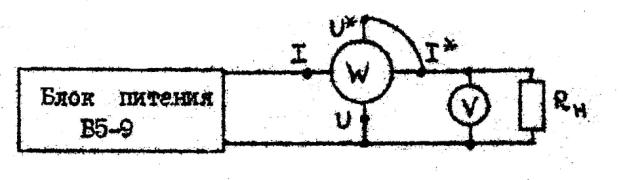
\includegraphics[width=\textwidth]{Part2.png}\\
	При измерении мощности устанавливают на нагрузке напряжение $U_{Н}$=40 В, которое измеряют вольтметром V. После этого измерения сопротивление нагрузки $R_{Н}$ и регистрирует показания ваттметра W. Результат измерения заносят в ф.2:\\

	\begin{table} [h!]
 	 	\begin{tabular}{|p{6cm}|p{2cm}|p{2cm}|p{2cm}|p{2cm}|}
		 	\hline
		 	Напряжение $U_{H}$, (В) & 40 & 40 & 40 & 40 \\
		 	\hline
		 	Сопротиаление $R_{H}$, (Ом) & 500 & 1000 & 1500 & 2000 \\
		 	\hline
		 	Показания ваттметра $P_{w}$, (Вт) & 3.4 & 1.2 & 0.7 & 0.4 \\
		 	\hline
		 	Поправка - $\Delta _{P}$, (Вт) & 0.15 & 0.15 & 0.15 & 0.15 \\
		 	\hline
		 	Мощность нагрузки $P_{H}$, (Bт) & 3.25 & 1.05 & 0.55 & 0.25 \\
		 	\hline
		 	Погрешность $\delta _{p}$, (\%) & 2.2 & 6.25 & 10.7 & 18.75 \\
		 	\hline
 		\end{tabular}
	\end{table}

 	\vspace{1cm}

 	Сопротивление нагрузки: $R_{H}$=100 кОм.\\
 	Мощность $P_{Н}$ , потребляемую нагрузкой, вычисляют по формуле $Р_{Н}$ =$P_{w}$ - $\delta$Р.\\
 	Относительную погрешность измерения мощности рассчитывают по формуле:\\
 	$\delta _{p}$ = ($U_{H}$*$I_{H}$*$k_{w}$ / $P_{w}$) * 100\%

